\documentclass[letterpaper,11pt]{article}
\usepackage[utf8]{inputenc}
\usepackage[bottom]{footmisc}
\usepackage{graphicx}
\usepackage{amsmath}
\usepackage{amsthm}
\usepackage{amscd}
\usepackage{amssymb}
\usepackage{latexsym}
\usepackage{upref}
\usepackage[hidelinks]{hyperref}
\usepackage{cite}
\usepackage{subcaption}

\setlength{\textwidth}{6.4in}
\setlength{\textheight}{9.5in}
\setlength{\topmargin}{-1in}
\addtolength{\headheight}{0.0675in}
\setlength{\oddsidemargin}{0.2in}
\setlength{\evensidemargin}{0.2in}

\begin{document}

    \title{
        A Deep Learning Approach to Solving Convective PDEs\\
    }
    \author{%
        Thompson, J.
    }
    \date{\today}
    \maketitle

    \begin{abstract}
        In this project, we examine a deep learning approach to solving various hyperbolic equations, including 
        (but not limited to) a basic advection equation and the one-dimensional viscous Burgers equation.
        Such equations arise naturally in the study of fluid and traffic flows and are solvable via traditional 
        finite difference approaches. Numerical solutions are therefore readily available (or may be easily generated),
        and so the problem of data collection for deep learning is well-mitigated.
    \end{abstract}


    \section{Background}\label{sec:background}
    Recent advancements in the field of machine learning have led to the development of Physics-Informed Neural 
    Networks (PINNs), wherein a neural network is used as a solution surrogate to systems of partial differential 
    equations (PDEs). Such networks are typically trained from available sparse data; typically, the amount of data
    available to train a neural network is insufficient for a neural network to converge. However, by encoding the 
    governing PDE term into the network training process (either by including the PDE residual into network training as
    in a multi-objective approach or by some other scheme), recent empirical successes indicate that
    sparse data and/or specified boundary conditions provide sufficient convergence conditions for the neural network to
    successfully approximate the true PDE solution.\cite{raissi_physics-informed_2019} In fact, neural networks are 
    particularly well-suited to solve the inverse problem for PDEs - that is, to infer some unknown parameter of 
    function which is part of the original system of PDEs.\cite{lu_deepxde_2021} In this project, we utilize PINNs to 
    solve both the forward and inverse problem for two well-known convective PDEs. The first of these is the standard 
    advection equation, which is perhaps the simplest possible hyperbolic PDE:

    $$
    u_t + a u_x = 0
    $$

    \ \\
    \noindent for some constant $a$ and initial condition $u(x, 0) = u_0(x)$. The second equation we will examine is the
    viscous Burgers' equation, which we obtain by letting $a = u$ from above and introducing a diffusive term 
    $\nu u_{xx}$:

    $$
    u_t + u u_x = \nu u_{xx}
    $$

    \section{Methodology}\label{sec:proposed-methodology}

    In this project, we utilize DeepXDE\footnote{
        Source code for this library may be found at
        \hyperlink{https://github.com/lululxvi/deepxde}{https://github.com/lululxvi/deepxde}
    }, a Python framework built on top of Tensorflow for scientific machine learning and physics-informed 
    learning.\cite{lu_deepxde_2021} DeepXDE solves PDEs by embedding the PDE residual term into the loss term of the
    neural network solution approximation. For the forward solution (i.e., with specified initial and boundary 
    conditions), the resulting neural network takes spatiotemporal data as input and outputs the predicted solution 
    value at each point. PINNs typically operate well with 1-3 hidden layers, though one aim of this project is to 
    determine which neural network architecture(s) lead to convergent system solutions. For the inverse problem, we will
    generate training data for both advection and inviscid Burgers' equations via known solutions for particular values
    of $a$ and initial condition $u_0(x)$ to determine these values from sampled solution data. In general, we 
    define a general non-linear partial differential equation as follows:

    $$
    u_t + N[u; \lambda] = 0, x \in \Omega, t \in [0, T]
    $$

    \ \\
    \noindent where $u(x, t)$ solves the PDE, $N[\cdot, \lambda]$ denotes some non-linear differential operator, and 
    $\lambda$ may represent some unknown (learnable) parameter(s) in the non-linear PDE. To determine a numerical PINN 
    solution to the PDE, we substitute a neural network $\mathcal{NN}(x, t; \lambda)$ solution surrogate for $u(x, t)$. 
    We do so by utilizing \textit{multi-task learning}, wherein we optimize for two distinct objectives. The first of 
    these objectives - unique to PINNs - is to minimize the PDE residual:

    $$
    L_{res} = ||u_t + N[u; \lambda]||
    $$

    \ \\
    For the PDEs discussed at present, we will find that this loss term (when encoded with appropriate boundary 
    conditions) is often sufficient to solve the PDE in the forward case. When observed measurement data for the PDE 
    is available (perhaps by way of some physical sensor array), we may utilize an additional, more conventional loss 
    term which penalizes the neural network solution for failing to satisfy observed measurements:

    $$
    L_{obs} = ||u - \hat{u}||_{\Gamma}
    $$

    \noindent where $\hat{u}$ represents (generally sparse) measured data at various points 
    $\Gamma \in \partial \Omega \cup \Omega$ in the domain. In general, then, our problem reduces to finding appropriate
    neural network parameters $\lambda$ which minimize this aggregate loss:
    
    \begin{equation}
        \min_{\lambda}{L_{obs} + L_{res}}
    \end{equation}

    We do so first by way of the Adam\cite{adam} algorithm to find candidates for global minima and then L-BFGS to 
    narrow in on our solution candidate. Lastly, we utilize the hyperbolic tangent activation function in our neural 
    network in order to satisfy smoothness requirements for PDEs.

    \section{Advection Equation}{\label{sec:advection-equation}}
    We begin with the 1D advection equation. This equation serves as a useful model for describing the movement of some
    material by way of ambient fluid velocity. If we suppose that our system takes place in a one-dimensional donut and
    wrap our domain in a circle (with the assumption that advected material moves in a single direction), we ought to
    expect that such a system gives rise to a periodic boundary condition, i.e., $u(0, t) = u(1, t)$. Our problem
    statement then becomes:

    $$
    u_t + a u_x = 0, x \in [0, 1], t \in [0, 1]
    $$

    \noindent with boundary conditions

    $$
    u(0, t) = u(1, t), u(x, 0) = \eta(x)
    $$

    Solutions to this equation are given by:

    \begin{align*}
        u(x, t) = \eta(x - at)
    \end{align*}


    \subsection*{Forward Solution}{\label{sec:advection-equation-forwared}}
    To solve this equation via a PINN, we utilize a fully-connected neural network with three hidden layers and 12 
    neurons in each layer. Because we are solving this equation forward in time, we do not have any pre-existing 
    measurement data from which to train. As such, our optimization target reduces solely to the PDE residual and 
    corresponding boundary conditions.


    \begin{figure}[h]
        \centering
        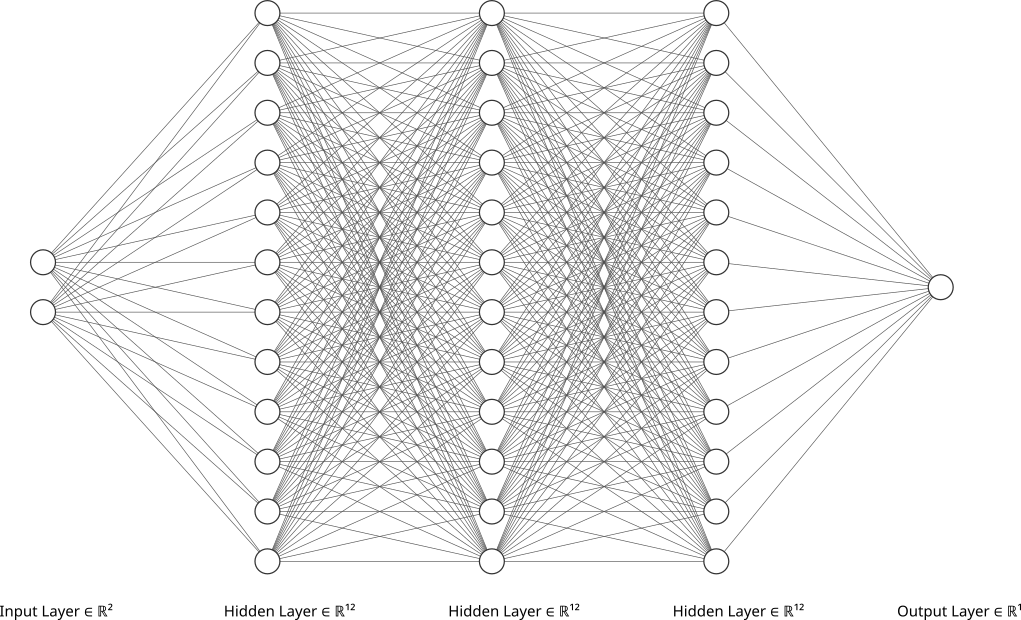
\includegraphics[width=0.70\textwidth]{nn.png}
        \caption{Advection equation network architecture with inputs $x, t$ and output $u$}
    \end{figure}

    We train our solution on a spatiotemporal grid with one spatial dimension and one temporal dimension. We train on 
    400 and 20 randomly sampled points from our domain; in general, these points may be arbitrary, though some degree of
    coverage of the domain facilitates a convergent solution over the entire domain. Training data is generated by 
    evaluating the PDE residual at each sampled point. Lastly, we impose a Gaussian initial condition:

    $$
    \eta(x) = e^{-(4x)^2},\; x \in [0, 1]
    $$
    
    We find that the neural network solution converges after 10000 iterations with a mean residual on the order of 
    $10^{-4}$ and L2 relative error on the order of $10^{-2}$. Of particular interest is the fact that the neural 
    network solution performs quite well outside the original temporal domain; in fact, we observe that while the neural
    network is trained to optimize the PDE residual on $t \in [0, 1]$, the learned solution closely matches the exact 
    solution up until $t=3$. This suggests that the neural network learns (to some degree) that solutions to the 
    advection equation consist of traveling wave packets.

    \begin{figure}[h]
        \centering
        \begin{subfigure}{0.45\textwidth}
            \includegraphics*[width=\textwidth]{advection_forward_t0.00.png}
            \caption{$t = 0$}
        \end{subfigure}
        \hfill
        \begin{subfigure}{0.45\textwidth}
            \includegraphics*[width=\textwidth]{advection_forward_t1.00.png}
            \caption{$t = 1$}
        \end{subfigure}
        \begin{subfigure}{0.45\textwidth}
            \includegraphics*[width=\textwidth]{advection_forward_t2.00.png}
            \caption{$t = 2$}
        \end{subfigure}
        \hfill
        \begin{subfigure}{0.45\textwidth}
            \includegraphics*[width=\textwidth]{advection_forward_t3.00.png}
            \caption{$t = 3$}
        \end{subfigure}
        \caption{Solution to $u_t + 0.4 u_x = 0$ with 20 temporal and 400 spatial points}
    \end{figure}

    \subsubsection*{Comparison with Finite Differences}
    Conservation equations are notoriously difficult to solve by standard numerical schemes due to the presence of
    discontinuous shock solutions. In particular, finite difference methods for the advection equation typically require
    careful discretization in order to prevent the introduction of numerical oscillations, damping, or instability.
    
    PINNs, as we shall see, handle this quite well. In particular, it is of interest to note that the formulation of 
    PINNs as a constrained optimization problem allows for arbitrary meshes from which to sample training points 
    \footnote{
        There is most assuredly some lower limit to this, though that limit naturally depends on the problem and domain 
        under consideration.
    }. As such, PINNs fall into the class of \textit{meshfree} numerical methods. In particular, this eliminates
    the need to correlate spatial and temporal discretizations in a particular way, e.g., by enforcing compliance with
    the Courant-Friedrichs-Lewy (CFL) condition for finite difference methods. We demonstrate this explicitly by 
    intentionally introducing an unstable finite difference grid by sampling $n^2$ spatial points - where $n$ is the 
    number of temporal points - in our domain; Figure 2 was generated with 20 temporal points and 400 spatial points.


    \subsection*{Inverse Solution}
    We now turn our attention toward solving the inverse problem, that is, given a PDE which presumably describes some
    observed phenomenon along with measurement data, we wish to learn one or more corresponding PDE parameters. To do 
    so, we require both a PDE candidate and a set of measured data which we require the PDE to satisfy so as to train
    a neural network to satisfy (1).
    
    It should be noted that the introduction of multiple training targets can sometimes introduce competing gradient 
    optimizations - in other words, satisfying $L_{obs}$ more closely sometimes incurs increased loss from the $L_{res}$
    term or vice versa. Such competition typically arises in one of two ways. The first and more obvious of these occurs
    when the PDE candidate does not accurately describe the physical phenomenon which gave rise to the observed data.
    The second of these tends to occur in multi-scale dynamic systems.\cite{pino} For the inverse problem, we 
    accordingly consider PDEs which are already scaled to unit domain.

    PINNs are particularly well-suited to solve the inverse problem. For the present purpose, we consider again the
    advection equation with unknown advection velocity $a$. As before, we utilize a fully-connected neutral network to 
    formulate a solution surrogate, but allow $a$ to represent a to-be-learned constant. Our inputs are therefore the
    spatial variable $x$, temporal variable $t$, and unknown velocity $a$. Given periodic boundary conditions and 
    initial condition $\eta(x)$ as before, we train the neural network for 15000 iterations with 10 data points computed
    from the exact solution at $t = 0.5$ with $a = 3$. We find that the neural network infers the correct advection 
    velocity to within 2\%.

    \begin{figure}[h]
        \centering
        \begin{subfigure}{0.45\textwidth}
            \includegraphics*[width=\textwidth]{advection_inverse_train_loss.png}
            \caption{Train loss for inverse advection problem}
        \end{subfigure}
        \hfill
        \begin{subfigure}{0.45\textwidth}
            \includegraphics*[width=\textwidth]{advection_inverse_learned_advection_velocity.png}
            \caption{Learned advection velocity}
        \end{subfigure}
        \caption{Inverse Advection Problem}
    \end{figure}

    \section{Burgers Equation}
    We now turn our attention away from the advection equation and toward solving a somewhat richer forward problem - 
    namely, we wish to solve the viscous Burgers equation:

    $$
    u_t + u u_x = \nu u_{xx}, x \in [-1, 1], t \in [0, 1]
    $$

    \noindent with boundary conditions

    $$
    u(-1, t) = u(1, t) = 0,\; u(x, 0) = -\sin{(\pi x)}
    $$

    In a similar fashion to the advection problem, we utilize a fully-connected neural network consisting of
    three hidden layers of 20 neurons each, which takes $x$ and $t$ as input and predicts the corresponding fluid 
    velocity $u$.  We observe that a shock begins to form approximately $t = 0.5$, and in particular that inaccuracies 
    occur around the point of discontinuity in the solution. To account for this, we implement residual-based adaptive 
    refinement (RAR) in order to re-train the network around specific points for which the PDE residual is 
    high.\cite{WU2023115671} To do so, we compute the maximum PDE residual after training in order to identify which 
    points contribute the most to the residual term. We then add these points to our training set and re-train the 
    network to account for these new points. We find that the solutions with and without residual-based adaptive 
    refinement agree with negligible difference at early timesteps (cf. Figures 
    \ref{burgers_forward_t0} vs. \ref{burgers_forward_t0_rar}), but the solution with RAR resolves small 
    inaccuracies at the region of steep gradient once the solution discontinuity begins to form at $t = 0.5$ 
    (cf. Figures \ref{burgers_forward_t0.5} vs. \ref{burgers_forward_t0.5_rar}).

    \begin{figure}[h]
        \centering
        \begin{subfigure}{0.45\textwidth}
            \includegraphics*[width=\textwidth]{burgers_forward_t0.00.png}
            \caption{$t = 0.00$ without RAR}
            \label{burgers_forward_t0}
        \end{subfigure}
        \hfill
        \begin{subfigure}{0.45\textwidth}
            \includegraphics*[width=\textwidth]{burgers_forward_t0.00_rar.png}
            \caption{$t = 0.00$ with RAR}
            \label{burgers_forward_t0_rar}
        \end{subfigure}
        \begin{subfigure}{0.45\textwidth}
            \includegraphics*[width=\textwidth]{burgers_forward_t0.50.png}
            \caption{$t = 0.50$ without RAR}
            \label{burgers_forward_t0.5}
        \end{subfigure}
        \hfill
        \begin{subfigure}{0.45\textwidth}
            \includegraphics*[width=\textwidth]{burgers_forward_t0.50_rar.png}
            \caption{$t = 0.50$ with RAR}
            \label{burgers_forward_t0.5_rar}
        \end{subfigure}
        \caption{Residual-based adaptive refinement for Burgers Equation}
    \end{figure}

    \section{Conclusions and Future Work}\label{sec:goals}
    In this report, we examined the efficacy of PINNs in computing forward solutions for the (upwind) advection equation
    and viscous Burgers equation. For the former, we found excellent agreement with the exact solution on the entire
    domain. Furthermore, we utilized the same neural network architecture as in the forward solution to learn the 
    unknown advection velocity, which again displayed excellent correlation with the exact solution.
    For the viscous Burgers equation, we utilized residual-based adaptive refinement in order to train the PINN solution
    on problematic solution points which exhibit a steep gradient in the solution in order to bette model highly 
    dynamic solutions. A natural next step from this work is to solve the inverse problem for the viscous Burgers 
    equation. Because the viscosity term in the Burgers equation is typically small, this inverse problem embodies an
    inverse multi-scale PDE. Utilizing techniques such as multi-scale Fourier feature networks may lead to improved 
    solution accuracy.\cite{Wang_2021} Lastly, PINNs trained in this work all embed the underlying system geometry into
    the learned network; these networks therefore typically only apply to the domains upon which they were trained. One 
    notable exception to this case is that of the forward advection equation solution, which suggests the possibility 
    that these networks may be trainable to solve systems outside the training domain and boundary conditions, perhaps 
    by way of point-cloud based neural networks and/or Fourier decomposition of initial conditions.\cite{Kashefi_2022}
    

    \pagebreak

    \bibliographystyle{plain}
    \bibliography{refs}


\end{document}
